%\documentclass[referee]{aa} % for a referee version
%\documentclass[onecolumn]{aa} % for a paper on 1 column  
%\documentclass[longauth]{aa} % for the long lists of affiliations 
%\documentclass[letter]{aa} % for the letters 
\documentclass{aa}
\usepackage{showyourwork}


%
\usepackage{graphicx}
%%%%%%%%%%%%%%%%%%%%%%%%%%%%%%%%%%%%%%%%
\usepackage{txfonts}
%%%%%%%%%%%%%%%%%%%%%%%%%%%%%%%%%%%%%%%%
%\usepackage[options]{hyperref}
% To add links in your PDF file, use the package "hyperref"
% with options according to your LaTeX or PDFLaTeX drivers.
%
\begin{document} 


   \title{Collision debris from a disruptive event}

   \author{M. Kenworthy
          \inst{1}
          \and
          Arttu Sainio
          \inst{2}
          \and
          Eric E. Mamajek
          \inst{3}
          \and
          Joeseph Masiero
          \inst{4}
          \and 
          Amy Mainzer
          \inst{4}
          \and
          Joeseph (Davy) Kirkpatrick
          \inst{4}
          \and 
          NEOWISE authorship list
          \inst{4}
          }

   \institute{Leiden Observatory, University of Leiden,
   PO Box 9513, 2300 RA Leiden, The Netherlands\\
   \email{kenworthy@strw.leidenuniv.nl}
         \and
             Arttu's address ...\\
    \and
    JPL
    \and
    Caltech/IPAC, 1200 E California Blvd, Mail Code 100-22, Pasadena, CA 91125, USA}

   \date{Received XXXX; accepted XXXX}

% \abstract{}{}{}{}{} 
% 5 {} token are mandatory
 
  \abstract
  % context heading (optional)
  % {} leave it empty if necessary  
   {Collisions occur between planetessimals that generate debris disks throuhg collisional cascades.}
  % aims heading (mandatory)
   {We analyze the dust and size distribution of the eclipse seen towards ASASSN-21qj.}
  % methods heading (mandatory)
   {Fit the light curve from three different colours to determine the particle size and distribution.}
  % results heading (mandatory)
   {The eclipse is coloured, indicating dust.
   %
   The dust has a lower limit mass of XXXX Earths, elcipse has a duration of XXXX days.}
  % conclusions heading (optional), leave it empty if necessary 
   {}

   \keywords{giant planet formation --
                $\kappa$-mechanism --
                stability of gas spheres
               }

   \maketitle
%
%-------------------------------------------------------------------

\section{Introduction}

The star blah blah underwent an exgtended dimming event from 2021, announced by the ASAS-SN group in Atronomersd Telegram xxxxx.


Sainio noted that the star underwent a significant brightening in the NEOWISE photometry.

The brightening is indicative of a collisional event between planetessimals that generates a significant amount of smaller dust, which explains the brightening in W3 and W4 seen with the NEOWISE data.

The subsequent dimming seen by ASAS-SN shows the debris cloud passing in front of the star.


\section{Observatons}

\subsection{ASAS-SN photometry}
 \begin{figure}
   \centering
   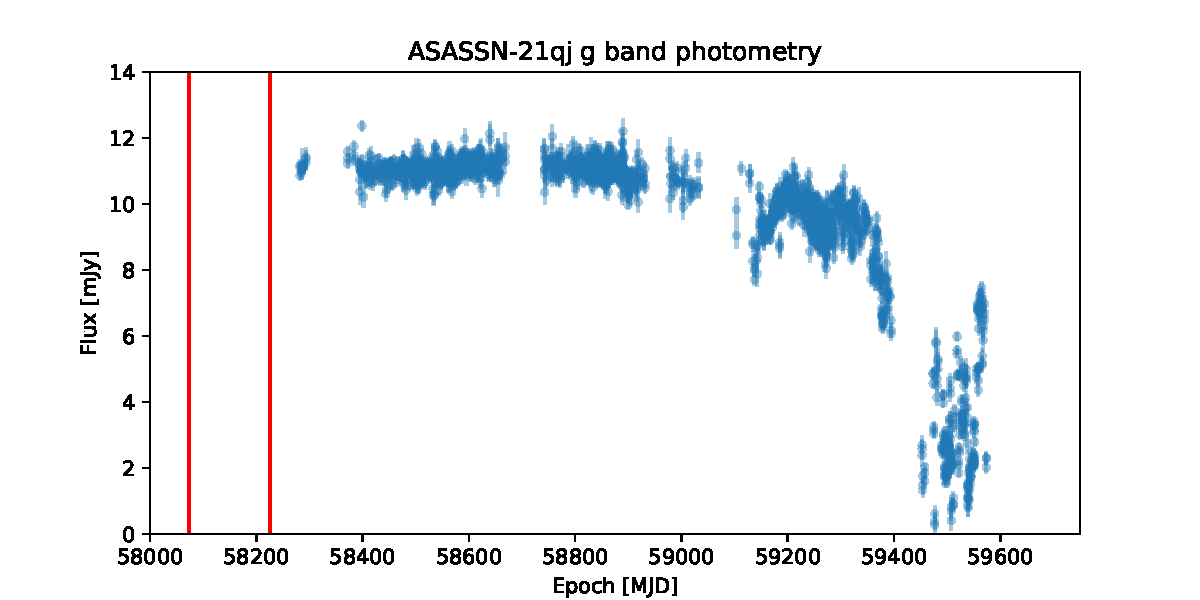
\includegraphics[width=\hsize]{ASAS-photometry.pdf}
      \caption{ASAS-SN $g'$ photometry of the star. The red lines indicate the epochs between which the NEOWISE brightening event occurred.
              }
         \label{fig:asphot}
   \end{figure}

\subsection{NEOWISE photometry}

\begin{figure}
   \centering
   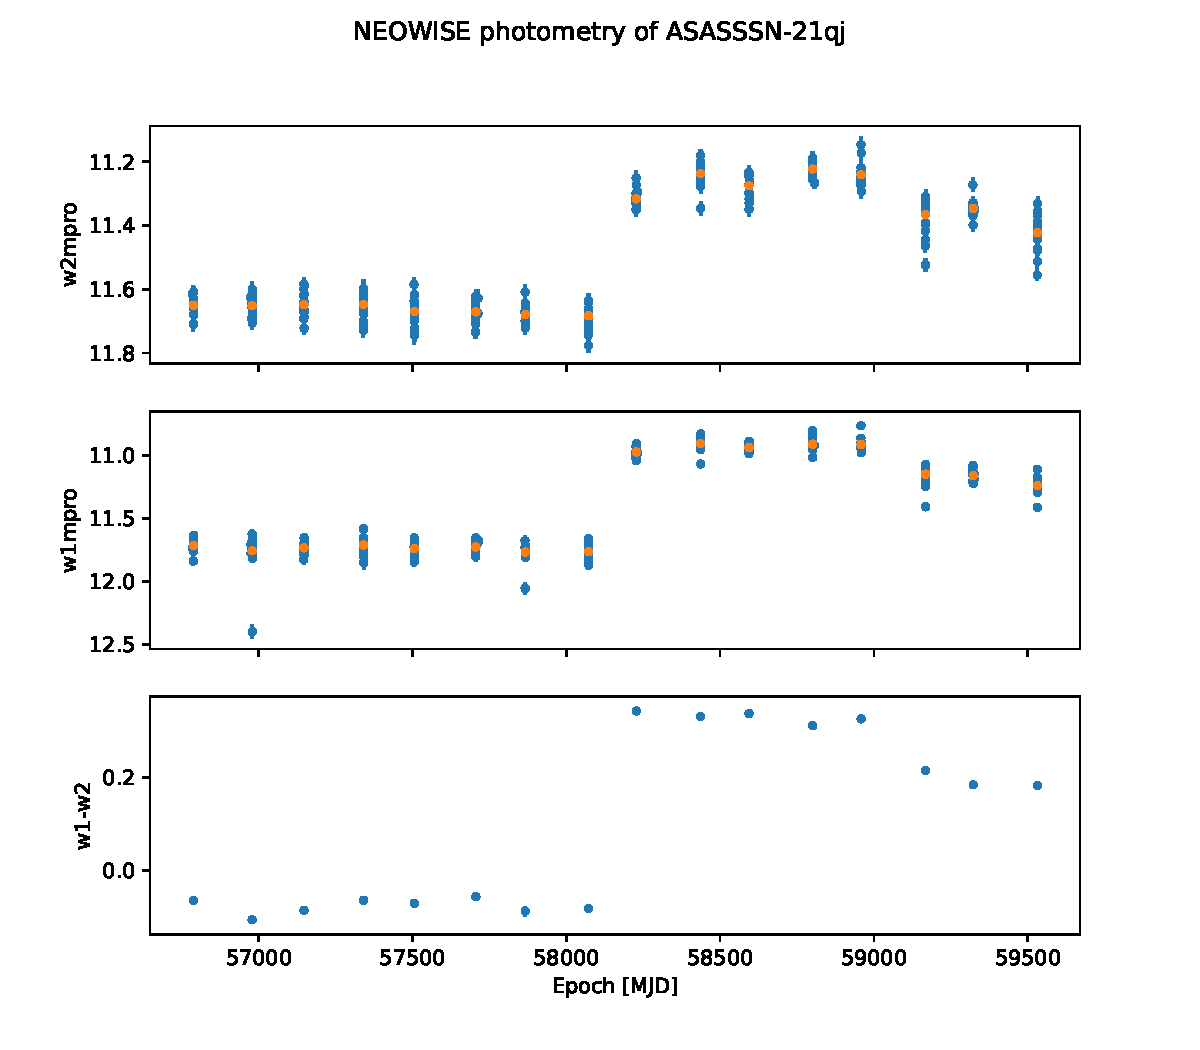
\includegraphics[width=\hsize]{NEOWISE_ASASSN-21dj.pdf}
      \caption{NEOWISE $W1$ and $W2$ photometry of the star, with the WISE color in the lowest panel.
      %
      A significant brightening event occurs between MJD 558074 and MJD 58225.
      %
      The $NEOWISE$ color changes from colourless to very red, which fades back towards colourless over 500 days.
              }
         \label{fig:wisephot}
   \end{figure}
   
\subsection{LCOGT photometry}

\subsection{ATLAS}

ATLAS photometry was obtained from their database.
ATLAS is a project that searches for near earth asteroids down to a magnitude of 19 
\citep{Tonry18}.
%
Two filters were obtained, the `o' and `c' filters respectively.
%
Photomety consists of two to four photometric points observed each night when conditions permitted.
%
Photometry with large errors was rejected in a first pass.
%
The remaining observations during a night were averaged and an error based on the r.m.s. of these nightly points was calaulated.
%
This left XXXx points covering from XXXX MJD to XXXX MJD.
%
The photometry covers the time period where the collision event occurred. 

\section{Properties of the star}

SED from Eric and VOSA in Figure~\ref{fig:sed}.

 Including IR WISE photometry
was forcing it to lower metallicity ([Fe/H] ~ -0.5-1), cooler (~Sun) fits. Fits also favor low reddening values (Av ~ 0.05). 
Similar to Alpha Cen A, but ~solar metallicity seems OK now. Almost exactly 1 Rsun! 

Best parameters as of 1/2/2022 (see below from VOSA fit) 
Teff = 5900 +- 74 K
log(L/Lsun) = 0.046+-0.013 
Av = 0.05+-0.03
mbol = 13.39+-0.02 (apparent)
logg = 4.5+-0.25
[M/H] = 0.0+-0.23 
Rad = 1.009 +- 0.030 Rsun


\begin{figure}
   \centering
   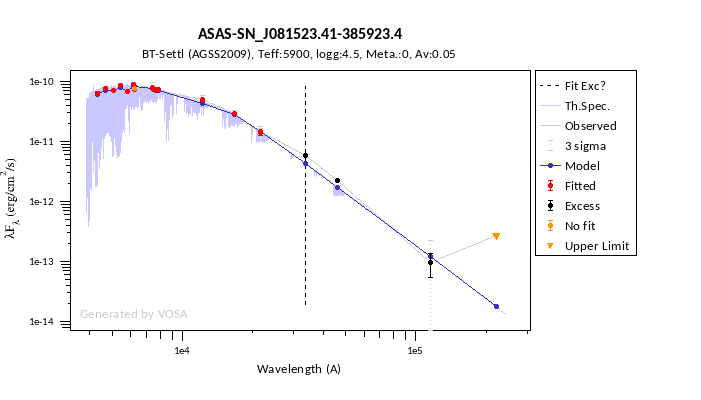
\includegraphics[width=\hsize]{ASAS-SN_J081523.41-385923.4.bt-settl-agss.5881.phot.png}
      \caption{VOSA fit to photometry of ASAS-SN J0815.}
         \label{fig:sed}
   \end{figure}


\section{Analysis}

\subsection{dust properties from the colors}

\section{Discussion}

Cound be a ring system

Could be a planetessimal system evolving

Something else?


%------------------------
\section{Conclusions}

   \begin{enumerate}
      \item There was a collision between planetoids towards ASASSN-21qj which generated a debris cloud.
      \item The cloud moved in front of the star, and we have a fresh measure of the debris from a collision.
   \end{enumerate}

\begin{acknowledgements}
      Part of this work was supported by the German
      \emph{Deut\-sche For\-schungs\-ge\-mein\-schaft, DFG\/} project
      number Ts~17/2--1.
\end{acknowledgements}

% WARNING
%-------------------------------------------------------------------
% Please note that we have included the references to the file aa.dem in
% order to compile it, but we ask you to:
%
% - use BibTeX with the regular commands:
%   \bibliographystyle{aa} % style aa.bst
%   \bibliography{Yourfile} % your references Yourfile.bib
%
% - join the .bib files when you upload your source files
% -------------------------------------------------------------------
\bibliographystyle{aa}
\bibliography{bib}

\end{document}
